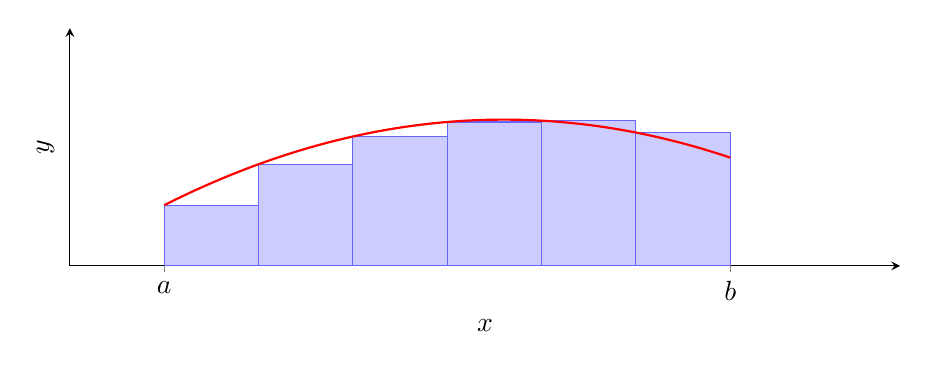
\begin{tikzpicture}
      \begin{axis}[width=\textwidth,height=4.6cm,axis lines=left,
        xlabel={$x$},ylabel={$y$},xmin=0,xmax=4.4,ymin=0,ymax=4.5,
        xtick={0.5,3.5},xticklabels={$a$,$b$},ytick=\empty]
        \addplot[ybar interval,fill=blue!20,draw=blue!60,domain=0.5:3.5,samples=7]
          {1+0.25*(x-0.5)*(3.5-x)*2+0.3*x};
        \addplot[thick,red,domain=0.5:3.5,samples=60]{1+0.25*(x-0.5)*(3.5-x)*2+0.3*x};
      \end{axis}
    \end{tikzpicture}